\documentclass[a4paper]{article}

\usepackage[margin=1in]{geometry} 
\usepackage{amsmath,amsthm,amssymb, graphicx, multicol, array, tikz}
\usetikzlibrary{automata, positioning}

\pdfminorversion=7
\pdfsuppresswarningpagegroup=1

\newcommand{\R}{\mathbb{R}}
\newcommand{\N}{\mathbb{N}}
\newcommand{\Z}{\mathbb{Z}}
\newcommand{\beh}{\textit{Behauptung. }}

\setlength{\parindent}{0pt}
\newenvironment{Aufgabe}[2][Aufgabe]{\begin{trivlist}
\item[\hskip \labelsep {\bfseries #1}\hskip \labelsep {\bfseries #2.}]}{\end{trivlist}}


\begin{document}
\begin{center}
	\section*{Langzeitverhalten von Markowketten - Handout}
\end{center}

Im Folgenden schauen wir uns ausschließlich Markowketten mit endlich vielen Zuständen an.
Wir betrachten immer einen Zustandsraum $I$ mit $n \in \mathbb{N}$ Zuständen.
Also können wir uns immer die Übergangsgraphen anschauen und auch die Übergangsmatrizen,
welche wie folgt aussehen:

\[
\mathbb{P} = \begin{pmatrix} 
	p_{11} & \cdots & p_{1n} \\
	\vdots & \ddots & \vdots \\
	p_{n1} & \cdots & p_{nn}
\end{pmatrix} 
\text{ wobei für alle $0 \leq j \leq n$ gilt }
\sum_{i=1}^{n} p_{ji} = 1
\]
Wir erinnern uns, dass diese Matrix die Wahrscheinlichkeiten beschreibt von einem Zustand $i$ in einen
Zustand $j$ zu gelangen. Wohlgemerkt betrachten wir nur homogene Markowketten, sodass diese Wahrscheinlichkeit
zu jedem Zeitpunkt die selbe ist.

\section{Invariante Wahrscheinlichkeitsverteilung}
Wir schauen uns Markowketten für die wir ein $L \in \mathbb{N}$ finden können, sodass
wir in $L$ Schritten von jedem Zustand in jeden anderen Zustand gelangen können.
Das heißt dann also für unsere Übergangsmatrix:
\[
\mathbb{P} ^{L} > 0
\] 
Diese Notation meint, dass alle Einträge der Matrix $\mathbb{P}$ hoch $L$ strikt positiv sind.
Wenn unsere Markowkette diese Bedingung erfüllt, dann können wir zeigen, dass es einen
Wahrscheinlichkeitsvektor $\rho$ gibt welcher folgende Bedingung erfüllt:

\[
\rho_k = \sum_{j=1}^{n} \rho_j p_{jk} \quad k \in I
\]

Diesen Wahrscheinlichkeitsvektor nennen wir dann \textit{invariante Verteilung}.
Wir beobachten, dass dieser letztendlich Aufschluss über die Wahrscheinlichkeit gibt, dass sich die
Markowkette in einem bestimmten Zustand $k$ befindet.

\section{Kommunizierende Zustände und Periodizität}

Um den Begriff der 'kommunizierenden' Zustände zu erläutern betrachten wir Folgende Markowkette.

\begin{center}
	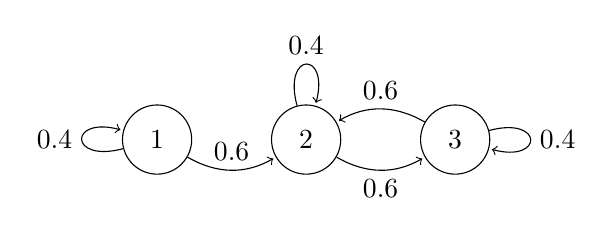
\begin{tikzpicture}
		% Add the states
		\node[state]			 (a) {1};
		\node[state, right=of a] (b) {2};
		\node[state, right=of b] (c) {3};

		% Connect the states with arrows
		\draw[every loop]
			(a) edge[bend right, auto=left]  node {0.6} (b)
			(b) edge[bend right, auto=right] node {0.6} (c)
			(c) edge[bend right, auto=right] node {0.6} (b)
			(a) edge[loop left]			 node {0.4} (a)
			(b) edge[loop above]			 node {0.4} (b)
			(c) edge[loop right]			 node {0.4} (c);
	\end{tikzpicture}
\end{center}
\qquad \caption{\textbf{Abbildung 1.1:} Eine Markowkette ohne invariante Verteilung}
\\

Uns fällt direkt auf, dass wir für diese Kette keine invariante Verteilung finden werden. 
Denn sobald wir einmal den Zustand 1 verlassen, haben wir keine Möglichkeit in diesen wieder
zurückzukehren.
Schauen wir uns die korrespondierende Übergangsmatrix an:
\[
\mathbb{P} = \begin{pmatrix} 
	0.4 & 0.6 & 0 \\
	0 & 0.4 & 0.6 \\
	0 & 0.6 & 0.4
\end{pmatrix} 
\]

Wir sehen, dass für alle $L \in \mathbb{N}$ der Wert in $(\mathbb{P} ^{L}) _{j1} = 0, j \in \{
	2, 3
\} $. 
Denn wir haben auch nach $L$ Schritten immer noch keine Möglichkeit wieder in Zustand 1 zu gelangen.
\\

Wir schreiben für zwei Zustände $i$ und $j$: $i \leadsto j [n]$ falls es ein $n \in \mathbb{N}$ gibt, sodass
der Zustand $i$ in $n$ Schritten zu $j$ führt. Dann schreiben wir verkürzt auch $i \leadsto j$.
Folglich sagen wir, dass die Zustände $i$ und $j$ kommunizieren, falls $i \leadsto j$ und auch
$j \leadsto i$, dann schreiben wir
\[
	i \leftrightsquigarrow j \quad \text{($i$ \textit{kommuniziert} mit $j$)}.
\]
Des weiteren nennen wir einen Zustand $i$ \textit{wesentlich}, wenn jeder Zustand $j$ zu dem $i$ führt, auch
zurück zu $i$ führt. 
\\

Wir betrachten nun die \textit{Periodizität}  einer Markowkette.
Wir schauen uns einen Zustand $i$ an. Für diesen Zustand definieren wir
\[
d_i = \text{ggT} \{
	n \in \mathbb{N} : i \leadsto i[n]
\}
\] 
als die sogenannte \textit{Periode} von $i$.
Zustände für die $d_i = 1$ gilt nennen wir aperiodisch.
Analog nennen wir die Kette aperiodisch bzw. periodisch mit Periode $d$, wenn alle Zustände die selbe
Periode haben.
\\

Periodische Markowketten können wir wie folgt zerlegen.

\begin{center}
	\begin{tikzpicture}
		% Add the states
		\node[state]			 (a) {1};
		\node[state, right=of a] (b) {2};
		\node[state, right=of b] (c) {3};
		\node[state, right=of c] (d) {4};
		\node[state, right=of d] (e) {5};

		% Connect the states with arrows
		\draw[every loop]
			% a -> b -> c -> d
			(a) edge[bend right, auto=right] node {} (b)
			(b) edge[bend right, auto=right] node {} (c)
			(c) edge[bend right, auto=right] node {} (d)
			(d) edge[bend right, auto=right] node {} (e)

			% d -> c -> b -> a
			(e) edge[bend right, auto=right] node {} (c)
			(c) edge[bend right, auto=right] node {} (a)
	\end{tikzpicture}
\end{center}
\qquad \caption{\textbf{Abbildung 1.2:} Eine periodische Markowkette}
\\

Nun erkennen wir, dass die obige Markowkette Periode 3 besitzt.
Wählen wir beispielsweise Zustand 1 aus, so beobachten wir, dass wir den restlichen Teil der Markowkette
in Folgende Teilmengen zerlegen können.
\[
	C_0(1) = \{
		1, 4
	\}, \; C_1 (1) = \{
		2, 5
	\}, \; C_2 (1) = \{
		3
	\} 
\]

\section{Rekurrenz und Transienz}
Wir nennen einen Zustand $i$ \textit{rekurrent} wenn dessen Markowkette immer wieder zu ihm zurückkehrt.
Andernfalls nennen wir ihn \textit{transient}.
Analog nennen wir eine Markowkette \textit{rekurrent} beziehungsweise \textit{transient} wenn alle Zustände
\textit{rekurrent} beziehungsweise \textit{transient} sind.
\\

Rekurrente Markowketten sind also genau die Markowketten für welche wir eine invariante Verteilung finden
können. Denn genau dann ist es ja nach $L$ Schritten möglich von jedem Zustand in jeden anderen Zustand
zu gelangen. Also auch insbesondere von jedem Zustand $i$ wieder zurück zu diesem.

\begin{center}
	\begin{tikzpicture}
		% Add the states
		\node[state]			 (a) {1};
		\node[state, right=of a] (b) {2};
		\node[state, right=of b] (c) {3};
		\node[state, right=of c] (d) {4};

		% Connect the states with arrows
		\draw[every loop]
			% a -> b -> c -> d
			(a) edge[bend right, auto=right] node {} (b)
			(b) edge[bend right, auto=right] node {} (c)
			(c) edge[bend right, auto=right] node {} (d)

			(d) edge[bend right, auto=right] node {} (c)
			(b) edge[bend right, auto=right] node {} (a)
			(a) edge[loop left] node {} (a)
			(d) edge[loop right] node {} (d)
	\end{tikzpicture}
\end{center}
\qquad \caption{\textbf{Abbildung 1.3:}  Eine transiente Markowkette}
\\

In diesem Fall können wir für die Zustände $1$ und $2$ eine erwartete Anzahl an Besuchen berechnen,
da diese ja endlich sind wenn wir die Markowkette unendlich lange simulieren lassen.

\end{document}
